\documentclass[aspectratio=169,14pt,usenames,dvipsnames]{beamer}

\usepackage[utf8]{inputenc}
\usepackage{fontspec}
\usepackage{enumitem}
\usepackage{calc}

\usepackage{datetime}
\newcommand\builddate{%
   \ifcase \month%
        \or Janeiro%
        \or Fevereiro%
        \or Março%
        \or Abril%
        \or Maio%
        \or Junho%
        \or Julho%
        \or Agosto%
        \or Setembro%
        \or Outubro%
        \or Novembro%
        \or Dezembro%
    \fi\space\number\year%
}

\newcommand{\loadtheme}[1]{%
    \input{themes/#1}%
}
\newcommand{\presentationlanguage}[1]{%
    \usepackage[#1]{babel}%
}

\newcommand{\usecodingsamples}[1]{%
    \usepackage{listings}%
    \input{listings/#1}%
}

% Configura a apresentação para ser executada em tela cheia.
\newcommand{\setfullscreen}{\hypersetup{pdfpagemode=FullScreen}}

% Hide beamer navigation simbols
\beamertemplatenavigationsymbolsempty

%
% Standard frames
%

% coverframe
\newcommand{\coverframe}{%
    \begin{frame} %
        \titlepage %
    \end{frame} %
}

% finalframe{email}
\newcommand{\finalframe}[2][Thank you!]{%
    \begin{frame}%
        \begin{flushright}%
            \huge \textbf{#1}%
            \vfill%
            \large \textbf{#2}%
        \end{flushright}%
    \end{frame}%
}

% bigtitle{title}
\newcommand{\bigtitle}[1]{%
    \begin{frame}%
        \begin{center}%
            \Huge {#1}%
        \end{center}%
    \end{frame}%
}

% citation{cite}{author}
\renewcommand{\citation}[2]{%
    \begin{frame}%
        \begin{center}%
            \vspace{1cm}
            \large \textit{"#1"}\\%
            \vspace{1cm}
            \footnotesize {#2}%
        \end{center}%
    \end{frame}%
}

% bigimage{file}
\newcommand{\bigimage}[2][1.0]{%
    {%
        \usebackgroundtemplate{}%
        \begin{frame}%
            {%
            \makebox[\textwidth][c]{%
              \includegraphics[height=#1\paperheight, width=#1\paperwidth,%
                               keepaspectratio]{#2}%
              }%
            }%
        \end{frame}%
    }%
}


\loadtheme{photoroll}

\subtitle{Conceitos Básicos de Fotografia Digital}
\title{A Luz e o seu Controle}
\author{}
\institute{Rafael\textbf{Jeffman}\\\tiny{F O T O G R A F I A}}
\date{Abril de 2018}

\begin{document}

%01
\coverframe

%02
\begin{frame}
    \frametitle{A Luz}
    \begin{itemize}
      \item A luz é a matéria prima da fotografia.
      \item Controlando a luz, pode-se criar formas, profundidade, sentimento.
      \item Podemos controlar a direção, qualidade e intensidade da luz.
    \end{itemize}
\end{frame}

%03
\begin{frame}
    \frametitle{Direção da Luz}
    \begin{itemize}
      \item Modifica a forma como vemos um objeto.
      \item Pode determinar o \textit{sentimento} transferido pela imagem.
      \item As sombras geradas podem salientar ou esconder detalhes.
      \item Pode ser de cima, frontal, lateral, contorno ou contraluz.
    \end{itemize}
\end{frame}

%04
\begin{frame}
  \frametitle{Luz Frontal}
  \begin{itemize}
    \item É uma luz que vem por trás do fotógrafo.
    \item Produz poucas sombras.
    \item Produz cores mais profundas.
    \item Pouca informação sobre a forma.
    \item Reduz as texturas.
  \end{itemize}
\end{frame}

%05
\imagevertical{Luz Frontal}{images/front-light.jpg}

%06
\begin{frame}
  \frametitle{Luz Lateral}
  \begin{itemize}
    \item É uma luz que vem pelos lados do objeto fotografado.
    \item Produz fortes sombras.
    \item Revela texturas e formas.
    \item É uma luz mais \textit{dramática}.
  \end{itemize}
\end{frame}

%07
\imagevertical{Luz Lateral}{images/side-light.jpg}

%08
\begin{frame}
  \frametitle{Luz de Contorno}
  \begin{itemize}
    \item É uma luz que não vem diretamente por trás do objeto, mas vem em um angulo maior de 90$^o$ da câmera.
    \item Destaca o contorno do objeto.
    \item Aumenta as sombras no objeto, diminuindo os detalhes.
    \item As cores ficam fracas e não produz texturas.
  \end{itemize}
\end{frame}

%09
\imagevertical{Luz de Contorno}{images/contour.jpg}

%10
\begin{frame}
  \frametitle{Contraluz}
  \begin{itemize}
    \item É uma luz que vem diretamente por trás do objeto.
    \item Normalmente, faz com que o objeto vire uma silhueta.
    \item Dificulta a fotometria, sendo quase impossível o uso do modo automático.
  \end{itemize}
\end{frame}

%11
\imagevertical{Contraluz}{images/backlight.jpg}

%12
\imagevertical{Contraluz}{images/silhueta_luz_natural.jpg}

%13
\imagevertical{Contraluz}{images/silhueta.jpg}

%14
\begin{frame}
  \frametitle{Luz de Cima}
  \begin{itemize}
    \item É a luz do \textit{meio-dia}, vindo diretamente de cima.
    \item Gera fortes sombras nos rostos.
    \item Em geral, gera imagens de alto contraste.
    \item Quando vinda do sol, gera cores fortes.
  \end{itemize}
\end{frame}

%15
\imagevertical{Luz de Cima}{images/luz-cima.jpg}

%16
\begin{frame}
    \frametitle{Intensidade da Luz}
    \begin{itemize}
      \item A intensidade da luz não muda, a não ser que se mude a origem.
      \item A luz perde intensidade com relação ao quadrado da distância.
      \item Ou seja, cada vez que a distância da fonte dobra, a intensidade
      de luz que atinge o objeto é dividida por quatro.
      \item Nem sempre podemos controlar a fonte de luz, mas podemos controlar
      a posição do objeto e como capturamos a luz.
    \end{itemize}
\end{frame}

%17
\begin{frame}
    \frametitle{Controle da Intensidade da Luz}
    \begin{itemize}
      \item Controlamos a sensibilidade (ISO), a velocidade (\textit{shutter}),
      e a abertura (\textit{aperture}), permitindo que mais ou menos luz atinja o sensor.
      \item Se não permitimos luz suficiente de atingir o sensor, a imagem ficará sub-exposta.
      \item Se permitimos que um excesso de luz atinja o sensor, a imagem ficará superexposta.
    \end{itemize}
\end{frame}

%18
\imagevertical{Subexposição}{images/subexposicao.jpg}

%19
\imagevertical{Sobrexposição}{images/sobrexposicao.jpg}

%20
\imagevertical{Exposição Adequada}{images/correct_exposure.jpg}

%21
\begin{frame}
    \frametitle{Tons}
    \begin{itemize}
      \item Todo suporte fotográfico tem uma capacidade de registrar uma quantidade máxima de tons.
      \item A diferença entre o tom máximo e mínimo nos dá o \textbf{alcance dinâmico} ou \textbf{latitude}
      do suporte fotográfico.
      \item Medimos esse alcance dinâmico em \textit{stops}, sendo que a diferença de \textit{1-stop} é o dobro
      de luminosidade.
      \item Os filmes tinham alcance dinâmico de 5 a 10 \textit{stops}. Os melhores sensores atuais
      chegam a 12 ou 14 \textit{stops}, no \textit{ISO base}.
    \end{itemize}
\end{frame}

%22
\begin{frame}
    \frametitle{Sombras}
    \begin{itemize}
      \item São os tons mais baixos de uma imagem.
      \item É onde mais aparece o ruído.
      \item Os \textbf{pretos}, apresentam pouca ou nenhuma textura.
      \item As \textbf{sombras}, apresentam uma textura razoável, e as cores
      começam a se definir.
      \item Deixar os tons muito escuros pode \textbf{bloquear as sombras}, o que era
      um problema grave nos filmes negativos.
    \end{itemize}
\end{frame}

%23
\begin{frame}
    \frametitle{Altas Luzes}
    \begin{itemize}
      \item São os tons mais altos de uma imagem.
      \item As \textbf{altas luzes} ou \textbf{realces}, apresentam pouca textura e cores
      claras, mais ainda definidas.
      \item Os \textbf{brancos}, não apresentam texturas, e devem ser restritos a
      reflexões especulares, ou fontes de luz.
      \item Nos filmes positivos e sensores digitais, o branco puro não pode ser
      recuperado e fica completamente sem detalhes, mesmo com ajustes posteriores
      (\textbf{\textit{blown highlights}}).
    \end{itemize}
\end{frame}

%24
\imagevertical{Estouro das Altas Luzes}{images/blownhighlights.jpg}

%25
\begin{frame}
    \frametitle{Tons Médios}
    \begin{itemize}
      \item A maior parte de informação está nos tons médios da cena.
      \item As texturas e as cores são melhor definidas nesses tons.
      \item A exposição indicada pelo fotômetro da câmera, quando \textit{zerado},
      indica quais são os tons médios.
    \end{itemize}
\end{frame}

%26
\begin{frame}
    \frametitle{O Sistema de Zonas}
    \begin{itemize}
      \item Popularizado por Ansel Adams, é uma forma de visualizar e registrar
      tons em uma fotografia.
      \item Define 10 (ou 11) zonas que variam do preto (0) ao branco (9 ou 10).
      \item Cada zona tem o dobro de luminosidade da zona anterior.
      \item Utilizando o fotometro \textit{spot}, podemos identificar na cena, as
      zonas que serão obtidas na captura.
    \end{itemize}
\end{frame}

%27
\bigimage{images/zone-system.jpg}

%28
\imagevertical{\textit{O Sistema de Zonas}}{images/zone-system-color.jpg}

%29
\begin{frame}
    \frametitle{Texturas}
    \begin{itemize}
      \item Texturas são reveladas pela diferença de tonalidades.
      \item A zona 5, é a que apresenta maior detalhe nas texturas.
      \item Quanto mais próximo das zonas 0 e 10, menos texturas são obtidas.
    \end{itemize}
\end{frame}

%30
\begin{frame}
    \frametitle{\Large Cores e Texturas no Sistema de Zonas}
    \begin{center}
        \fbox{
\includegraphics[width=2cm]{images/zone0.jpg}}
        \fbox{
\includegraphics[width=2cm]{images/zone1.jpg}}
        \fbox{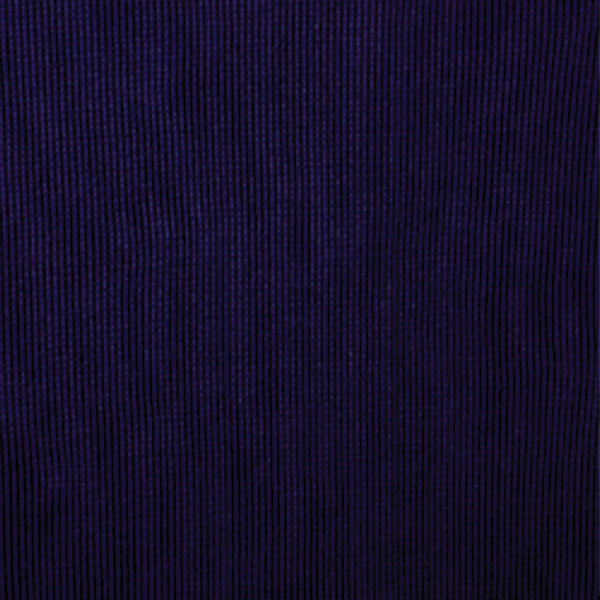
\includegraphics[width=2cm]{images/zone2.jpg}}
        \fbox{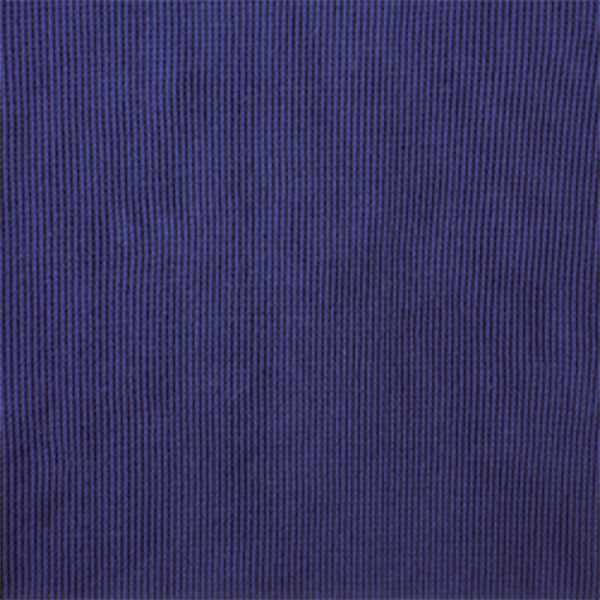
\includegraphics[width=2cm]{images/zone3.jpg}}
        \fbox{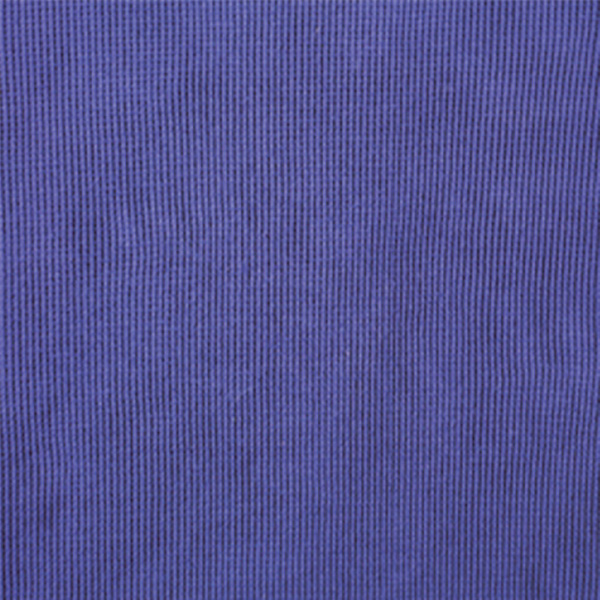
\includegraphics[width=2cm]{images/zone4.jpg}}

        \fbox{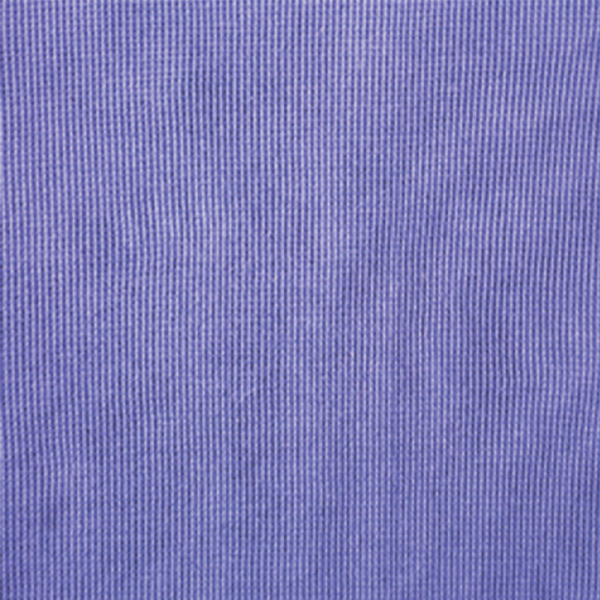
\includegraphics[width=2cm]{images/zone5.jpg}}

        \fbox{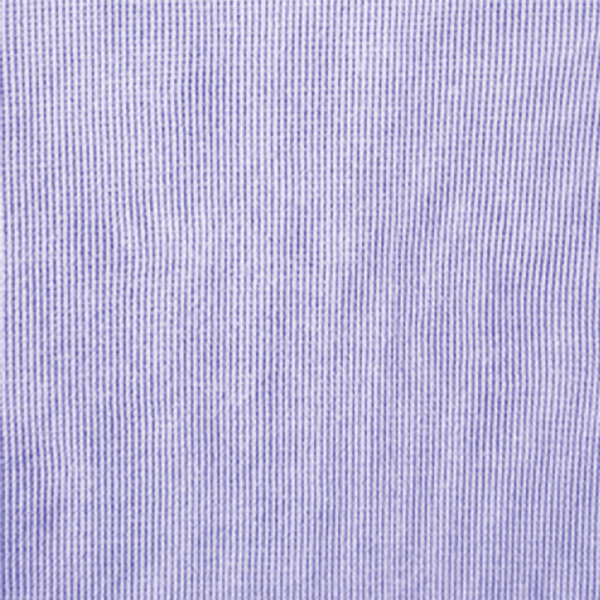
\includegraphics[width=2cm]{images/zone6.jpg}}
        \fbox{
\includegraphics[width=2cm]{images/zone7.jpg}}
        \fbox{
\includegraphics[width=2cm]{images/zone8.jpg}}
        \fbox{
\includegraphics[width=2cm]{images/zone9.jpg}}
        \fbox{
\includegraphics[width=2cm]{images/zone10.jpg}}
    \end{center}
\end{frame}

%31
\begin{frame}
    \frametitle{Cores e o Sistema de Zonas}
    \begin{itemize}
      \item A Zona 5 é a zona que permite mostrar cores mais saturadas.
      \item Nos filmes, a percepção de saturação é maior na Zona 4, o que não acontece nos sensores
      digitais (por terem um comportamento linear).
      \item Alguns sensores e filmes respondem com mais intensidade a algumas cores.
      \item Na fotografia digital, é possível recuperar a saturação de algumas cores,
      até certo ponto, reduzindo a exposição no processamento da imagem.
    \end{itemize}
\end{frame}

%32
\imagevertical{\textit{Cores e o Sistema de Zonas}}{images/zone-color-film.jpg}

%33
\begin{frame}
    \frametitle{\textit{High Key}}
    \begin{itemize}
      \item Estilo de fotografia onde a iluminação é utilizada para diminuir as
      sombras e contrastes.
      \item Surgiu como uma alternativa de iluminação em filmes, por as reproduções
      não lidavam bem com contrastes.
      \item Atualmente, é utilizado como estilo para mostrar positividade, inocência.
      \item \textbf{Não deve ser confundida com superexposição.}
    \end{itemize}
\end{frame}

%34
\imagevertical{\textit{High Key}}{images/highkey.jpg}

%35
\imagevertical{\textit{Sobrexposição!}}{images/High_key_overexposure.jpg}

%36
\begin{frame}
    \frametitle{\textit{Low Key}}
    \begin{itemize}
      \item Estilo de fotografia onde a iluminação é utilizada para enfatizar as
      sombras e contrastes.
      \item E utilizado como estilo para mostrar mistério, drama.
      \item É a base de iluminação para criar imagens \textit{Chiaroscuro}.
      \item \textbf{Não deve ser confundida com subexposição.}
    \end{itemize}
\end{frame}

%37
\imagevertical{\textit{Low Key}}{images/low-key.jpg}

%38
\begin{frame}
    \frametitle{Temperatura de Cor}
    \begin{itemize}
      \item Medida em Kelvin (K), está relacionada a distribuição de energia de luz
      irradiada por um "corpo negro".
      \item Valores mais altos, descrevem uma fonte de luz azulada.
      \item Valores mais baixos, descrevem uma fonte de luz azulada.
      \item A luz provida pelo sol varia de temperatura ao longo do dia.
    \end{itemize}
\end{frame}

%39
\imagevertical{Temperatura de Cor}{images/color-temperature-sun.jpg}

%40
\begin{frame}
    \frametitle{Cor e a Luz}
    \begin{itemize}
      \item Além da temperatura, a fonte luz pode variar em matiz, adicionando verde ou magenta
      à cena.
      \item Lampadas fluorescentes, principalmente antigas, adicionam tons esverdeados.
      \item Além da fonte de luz, a luz refletida por qualquer objeto colorido "assume" a cor
      daquele objeto.
      \item E nem toda fonte artificial de luz tem as mesmas propriedades com relação a
      reprodução de cores.
    \end{itemize}
\end{frame}

%41
\imagevertical{Cor e Luz}{images/white-balance.png}

%42
\begin{frame}
    \frametitle{\Large{Controle da Temperatura e Cor da Luz}}
    \begin{itemize}
      \item Pouco se pode fazer em relação ao controle da temperatura e a cor da luz,
      quando utilizamos a luz disponível (natural ou não).
      \item Para utilizar a luz disponível, com filmes, devemos utilizar filtros
      na objetiva, que corrigem a luz, para um tom neutro.
      \item Na fotografia digital,
        \begin{itemize}
          \item Podemos ajustar o tipo de luz na câmera.
          \item Podemos fotografar no formato \textbf{RAW}, e
          corrigir a temperatura e a cor da luz no processamento da imagem.
        \end{itemize}
    \end{itemize}
\end{frame}

%43
\begin{frame}
    \frametitle{Balanço de Branco}
    \begin{itemize}
      \item Para corrigir a cor durante a captura, é preciso ajustar o
      \textbf{balanço de branco} da câmera, para compensar a luz ambiente.
      \item Utilize o ajuste automático mais próximo das luzes do ambiente.
      \item Se você precisa de maior precisão, pode utilizar o modo personalizado.
      \item Ao fotografar em \textit{RAW}, o balanço de branco só afeta a imagem
      de \textit{preview}.
    \end{itemize}
\end{frame}

%44
\imagevertical{Modos de Balanço de Branco}{images/white-balance-presets.jpg}

%45
\begin{frame}
    \frametitle{Uso da Luz Natural}
    \begin{itemize}
      \item É uma luz que varia de intensidade e temperatura de cor, ao longo do dia.
      \item É uma luz que está em constante alteração de ângulo de incidência, porém,
      vem sempre de cima ou diretamente, nunca, por baixo.
      \item Possui uma excelente capacidade de reprodução de cores.
      \item Produz um luz levemente amarelada quando atinge diretamente o objeto,
      e uma luz azulada quando o atinge indiretamente.
    \end{itemize}
\end{frame}

%46
\begin{frame}
    \frametitle{Uso da Luz Disponível}
    \begin{itemize}
      \item A luz disponível inclui a luz natural e/ou a iluminação artificial disponível.
      \item Normalmente, não temos controle no posicionamento ou intensidade da luz.
      \item Em alguns ambientes, a iluminação é formada por diversas fontes de luz, com
      diferentes temperaturas de cor.
      \item Na maioria dos casos, tem uma capacidade de reprodução de cores razoável.
    \end{itemize}
\end{frame}

%47
\begin{frame}
    \frametitle{Uso do Flash}
    \begin{itemize}
      \item É uma luz com características semelhantes à luz natural.
      \item É fácil de controlar sua intensidade e posição.
      \item Podemos alterar a temperatura de cor utilizando filtros.
      \item Tem duração muito curta, mas, normalmente, limita a velocidade máxima do obturador.
      \item Possui uma excelente capacidade de reprodução de cores.
    \end{itemize}
\end{frame}

%48
\finalframe[Vamos gastar o obturador!]{rafasgj@gmail.com}

%49
\begin{frame}
    \frametitle{Bibliografia}
    \begin{itemize}
      \item \textbf{O Negativo}. Ansel Adams. Senac, 2004.
      \item \textbf{O novo manual de Fotografia}. John Hedgecoe. Senac, 2005.
    \end{itemize}
\end{frame}

\end{document}
